A person with a spinal cord injury who has lost control of his or her standing mechanism can potentially benefit from an external automatic control system that takes as input the desired leg angle and tries to control the actual leg angle, as shown in the figure below.
\begin{center}
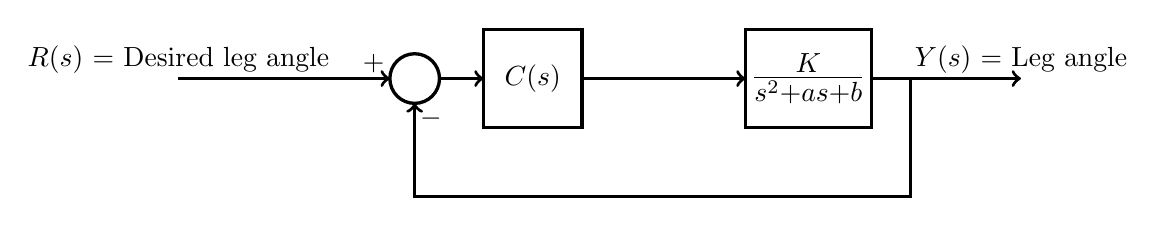
\begin{tikzpicture}[scale=1,inner sep=0pt,outer sep=0pt,very thick,
sysblock/.style={draw,rectangle,inner sep=2pt,minimum width=1.25cm,minimum height=1.25cm,very thick}]
\draw (2,0) node[draw,circle] (sum1) {$\rule{0pt}{18pt}$};
\draw (3.5,0) node[sysblock] (C) {$C(s)$};
\draw (7,0) node[sysblock] (G) {\Large $\frac{K}{s^2+as+b}$};
\draw[->] (-1,0) node[above=2pt] {$R(s)$ = Desired leg angle} -- (sum1.180) node[above left=2pt] {$+$};
\draw[->] (sum1.0) --  (C);
\draw[->] (C) -- (G);
\draw[->] (G) -- ++(2.7,0) node[above=2pt] {$Y(s)$ = Leg angle};
\draw[->] (G.0) ++(.5,0) -- ++(0,-1.5) -| (sum1.-90) node[below right=2pt] {$-$};
\end{tikzpicture}
\end{center}
In the plant transfer function, the parameters can change as the person's muscles tire out. 

(a) Sketch the root locus when using proportional control $C(s) = K_p$ for two cases: (i) (not tired) $K=10$, $a=12$, $b=100$, and (ii) (tired) $K=15$, $a=8$, $b=144$. Based on these two root locus plots, which case do you expect to result in higher percent overshoot in response to a step reference input for any given value of $K_p$?

(b) Create a Simulink model for both cases and use it to verify your answer to (a) when $K_p = 45$. (For Simulink help, see the PID control lecture.)

(c) What would be your next step to trying to reduce the percent overshoot? For example, would you change the gain $K_p$ or change the controller type to proportional-integral (PI) or proportional-derivative (PD)? Why?